%!TEX root = ./main.tex
\chapter{Implementación del Entorno de Desarrollo y Adquisición del Núcleo RISC-V}
\label{ch:implementacion_entorno}

Este capítulo describe el procedimiento metodológico seguido para la obtención, configuración del entorno de trabajo y empaquetado del procesador suave (\textit{soft-core}) RISC-V Ibex, asegurando su compatibilidad e integración posterior con las herramientas de diseño digital de Xilinx/AMD (Vivado), sentando las bases hardware para la arquitectura propuesta en esta tesis.

\section{Adquisición del Núcleo RISC-V Ibex}
Para la incorporación del núcleo de procesamiento \textit{open-source} en el sistema, se procedió a la clonación directa del repositorio oficial mantenido por LowRISC \url{https://github.com/lowrisc/ibex}. Los archivos fuente obtenidos fueron almacenados y descomprimidos en el directorio de trabajo destinado al desarrollo del proyecto en Vivado.

\section{Preparación y Configuración del Entorno de Herramientas (FuseSoC y Extracción)}
Con el propósito de mitigar posibles conflictos de dependencias en el sistema operativo host y aprovechar la compatibilidad con herramientas de compilación basadas en Unix, se configuró un entorno de desarrollo aislado utilizando el Subsistema de Windows para Linux (WSL con Ubuntu).

Dentro de dicho entorno, se inicializó un entorno virtual de Python denominado \textit{ibex\_env} mediante las siguientes directivas de consola:

\begin{lstlisting}[style=bashstyle]
root@DESKTOP-AD77AUU:~# python3 -m venv ~/ibex_env
\end{lstlisting}

Este enfoque de aislamiento garantiza la portabilidad del proyecto y previene incompatibilidades entre las librerías requeridas por los scripts de automatización de Ibex y las librerías globales del sistema operativo.



\section{Instalación y Verificación de FuseSoC}
Para proceder con la preparación de los archivos fuente del procesador, se activa previamente el entorno virtual de Python configurado:

\begin{lstlisting}[style=bashstyle]
source ~/ibex_env/bin/activate
\end{lstlisting}

A continuación, se instalan las dependencias de Python requeridas por el núcleo y la herramienta FuseSoC dentro del directorio de trabajo:

\begin{lstlisting}[style=bashstyle]
pip install -U -r python-requirements.txt
pip install --upgrade fusesoc
\end{lstlisting}

Una vez finalizada la instalación, se realiza una etapa de verificación de la correcta indexación de los núcleos mediante la consola de comandos:

\begin{lstlisting}[style=bashstyle]
fusesoc --cores-root . core list
\end{lstlisting}

Como resultado esperado de este comando, la consola deberá listar los núcleos disponibles en el repositorio, confirmando que FuseSoC reconoce el directorio actual como raíz de núcleos IP.

\subsection{Generación del Paquete para Vivado}
Para empaquetar y estructurar el núcleo RISC-V Ibex de forma compatible con la herramienta de síntesis, se ejecuta el comando de construcción de FuseSoC especificando el objetivo (\textit{target}) de análisis y configuración inicial:

\begin{lstlisting}[style=bashstyle]
fusesoc --cores-root . run --target=lint --setup --build-root ./build/ibex_out lowrisc:ibex:ibex_top
\end{lstlisting}

Una vez completado el proceso de compilación y empaquetado, los archivos fuente resultantes se encontrarán almacenados en la siguiente ruta relativa del proyecto:
\begin{center}
\texttt{ibex-master/build/ibex\_out/src/}
\end{center}

Este directorio contiene todos los archivos HDL y dependencias necesarias para importar el procesador suave dentro de un entorno de diseño en AMD/Xilinx Vivado.


\subsection{Entorno de Diseño con AMD Vivado}
Para la implementación y síntesis del hardware, se optó inicialmente por el uso de la herramienta AMD Vivado 2025.1. Sin embargo, durante las primeras etapas de desarrollo se identificaron múltiples incidencias e incompatibilidades en los bloques de Propiedad Intelectual (\textit{IP Cores}), lo cual motivó a utilizar Xilinx Vivado 2022.2 y Xilinx Vitis 2022.2.
%en una primera instancia el diseño rudimentario de una memoria instanciada por código. Si bien este enfoque incrementaba inicialmente la robustez ante futuras modificaciones o migraciones, pronto expuso limitaciones operativas significativas.

%El inconveniente principal radicó en la presencia recurrente de errores de software (\textit{bugs}) críticos asociados específicamente al bloque \textit{Block RAM} (BRAM). Ante la inviabilidad de continuar el desarrollo bajo estas condiciones de inestabilidad y con el fin de asegurar la reproducibilidad del sistema, se procedió a realizar un cambio de versión hacia una plataforma ampliamente probada y estable: \textbf{AMD Vivado 2022.2}, junto con su conjunto integral de herramientas complementarias, incluyendo \textit{Xilinx Vitis} para el desarrollo de software embebido.

El flujo de diseño combinó la utilización de diagramas de bloques (\textit{Block Design}) para la interconexión de componentes de alto nivel, complementado con el desarrollo de código HDL en etapas críticas del proyecto.

\section{Integración del Núcleo en Xilinx Vivado}
Con los archivos fuente generados y estructurados mediante FuseSoC, se procede a la integración en Vivado bajo el siguiente procedimiento metodológico:

\begin{enumerate}
    \item \textbf{Creación del Proyecto:} Se inicializa un nuevo proyecto en Vivado orientado a la placa de desarrollo objetivo Zynq 7000/ Zybo Z7.
    \item \textbf{Importación de Fuentes:} En la sección de adición de directorios (\textit{Add Directories}), se selecciona la carpeta contenedora de los fuentes generados previamente:
    
    \texttt{ibex-master/build/ibex\_out/src/}.
    
    \item \textbf{Definición del Nivel Superior:} Se designa explícitamente al archivo \textit{top-level} del núcleo (\texttt{ibex\_top.sv}) como el componente principal de jerarquía para las fases subsiguientes de síntesis y empaquetado de Propiedad Intelectual.
\end{enumerate}

\subsubsection{Subsistema Wrapper: \texttt{ibex\_bram\_subsystem}}
%Debido a la elevada cantidad de pines de entrada y salida expuestos de manera nativa por el núcleo Ibex, se implementó una estrategia de encapsulamiento mediante un componente \textit{wrapper}. Esta técnica permite abstraer las señales de control y buses que no son utilizados en la arquitectura actual, facilitando su integración en forma simplificada, limpia y funcional dentro del diagrama de bloques de Vivado.
 Siguiendo el esquema de encapsulamiento descripto en el capítulo \ref{ssec:wrapper_ibex} se configuraron los siguientes parámetros:

%Con el objetivo de dotar a este subsistema de autonomía para el almacenamiento y la ejecución de instrucciones de arranque (\textit{bootcode}) y datos iniciales, se instanció un bloque de memoria BRAM directamente en la misma jerarquía del envoltorio.

\paragraph{Configuración del Bloque BRAM:}
Para la configuración del bloque de memoria BRAM dentro del subsistema \textit{ibex\_bram\_subsystem}, se establecieron parámetros específicos en el asistente de IP de Vivado con el fin de garantizar la correcta compatibilidad con el bus de instrucciones y datos del núcleo Ibex. 

Los parámetros principales configurados en el generador de IP fueron los siguientes:

\begin{itemize}
    \item \textbf{Tipo de Memoria (\textit{Memory Type}):} Se seleccionó \textit{True Dual Port RAM}, lo que permite habilitar dos puertos de acceso independientes de lectura y escritura, facilitando la carga inicial de código y el acceso por parte del procesador.
    \item \textbf{Control de Algoritmo (\textit{Algorithm Options}):} Configurado en modo \textit{Low Power} para optimizar el consumo estático de los recursos lógicos de la FPGA.
    \item \textbf{Ancho de Datos (\textit{Write/Read Width}):} Ajustado a un ancho de $32$ bits, coincidiendo con el bus nativo de datos e instrucciones de la arquitectura RISC-V Ibex.
    \item \textbf{Profundidad de Memoria (\textit{Depth}):} Dimensionada de acuerdo con el espacio de direccionamiento requerido para las rutinas de arranque y el programa de prueba inicial (por ejemplo, un rango que permite almacenar el vector de reset y las primeras instrucciones del firmware).
    \item \textbf{Archivos de Inicialización (\textit{Load Init File}):} Se habilitó la carga de archivos de inicialización de memoria en formato hexadecimal (\textit{.mem} o \textit{.coe}), permitiendo que el núcleo comience a ejecutar instrucciones de manera autónoma desde el ciclo inicial de reloj tras el \textit{reset} del sistema.
\end{itemize}

Esta estructura de memoria interna asegura un acceso de baja latencia sin la necesidad de controladores externos complejos en las etapas iniciales de la síntesis del hardware.
A continuación \textit{ibex\_bram\_subsystem.sv} este scripts contiene la instanciacion de \textit{ibex\_top.sv} y BRAM configurada.

\begin{lstlisting}[style=verilogstyle, basicstyle=\ttfamily\footnotesize, caption={Codigo fuente del subsistema \texttt{ibex\_bram\_subsystem.sv}}, label={code:ibex_bram_subsystem}]
`timescale 1ns / 1ps

module ibex_bram_subsystem (
    input  wire        clk_i,      // Sincronizado con el clock de la ARM
    input  wire        rst_ni,     // Reset del Ibex controlado por el GPIO

    // --- INTERFAZ BRAM PROVENIENTE DEL AXI BRAM CONTROLLER (ARM) ---
    input  wire        bram_clk_a,   // Reloj del puerto A del controlador
    input  wire        bram_en_a,    // Enable del puerto A
    input  wire [3:0]  bram_we_a,    // Write Enable (byte-enables)
    input  wire [12:0] bram_addr_a,  // Direccion fisica 
    input  wire [31:0] bram_wdata_a, // Datos a escribir desde el ARM
    output wire [31:0] bram_rdata_a, // Datos leidos hacia el ARM

    // --- INTERFAZ EXTERNA HACIA EL REPORTER ---
    output wire        reporter_req_o,
    output wire [31:0] reporter_addr_o,
    output wire        reporter_we_o,
    output wire [31:0] reporter_wdata_o,
    input  wire [31:0] reporter_rdata_i
);

    // Senales internas del bus de instrucciones del Ibex
    logic        instr_req;
    logic [31:0] instr_addr;
    logic [31:0] instr_rdata;

    // Senales internas del bus de datos del Ibex
    logic        data_req;
    logic [31:0] data_addr;
    logic        data_we;
    logic [31:0] data_wdata;
    logic [31:0] data_rdata;

    logic [31:0] ram_rdata;
    logic        sel_ts; 

    // --- INSTANCIA DEL NUCLEO IBEX ---
    ibex_top #(                      // Instanciacion de Ibex.
        .PMPEnable ( 1'b0 ),
        .RV32E     ( 1'b0 ),
        .RV32M     ( ibex_pkg::RV32MFast )
    ) u_core_cpu (
        .clk_i          ( clk_i ),
        .rst_ni         ( rst_ni ),
        .test_en_i      ( 1'b0 ),
        .scan_rst_ni    ( 1'b1 ),
        .hart_id_i      ( 32'h0 ),
        .boot_addr_i    ( 32'h00000000 ),

        .instr_req_o    ( instr_req ),
        .instr_addr_o   ( instr_addr ),
        .instr_rdata_i  ( instr_rdata ),

        .data_req_o     ( data_req ),
        .data_addr_o    ( data_addr ),
        .data_we_o      ( data_we ),
        .data_wdata_o   ( data_wdata ),
        .data_rdata_i   ( data_rdata ),

        .irq_software_i ( 1'b0 ),
        .irq_timer_i    ( 1'b0 ),
        .irq_external_i ( 1'b0 ),
        .irq_nm_i       ( 1'b0 ),
        .debug_req_i    ( 1'b0 ),
        .fetch_enable_i ( 1'b1 )
    );

    // --- DECODIFICADOR PARA EL REPORTER ---
    assign sel_ts = (data_addr[31:28] == 4'h8);

    assign reporter_req_o   = data_req & sel_ts;
    assign reporter_addr_o  = data_addr;
    assign reporter_we_o    = data_we;
    assign reporter_wdata_o = data_wdata;

    assign data_rdata = sel_ts ? reporter_rdata_i : ram_rdata;

    // --- MULTIPLEXOR DEL PUERTO B DE LA BRAM ---
    logic        bram_portb_en;
    logic [3:0]  bram_portb_we;
    logic [31:0] bram_portb_addr;
    logic [31:0] bram_portb_wdata;
    
    // NUEVA SEnAL INTERMEDIA PARA ALINEAR LA ESCRITURA
    logic [3:0]  bram_portb_we_internal; 

    // REGLA DE ARBITRAJE:
    // Si data_we es 1 y NO estamos escribiendo en el Reporter
    // (!sel_ts), forzamos 4'b1111
    assign bram_portb_we_internal = 
    (!rst_ni) ? bram_we_a : ((data_we && !sel_ts) ? 4'b1111 : 4'b0000);

    // El Enable depende de data_req cuando el Ibex corre, no esta clavado en 1
    assign bram_portb_en    = (!rst_ni) ? bram_en_a    : data_req; 
    
    // Usamos la senal alineada
    assign bram_portb_we    = bram_portb_we_internal; 
    
    assign bram_portb_wdata = (!rst_ni) ? bram_wdata_a : data_wdata;
    
    // Mapeo de direcciones: Concatenamos 19 ceros + los 13 bits del ARM = 32 bits
    assign bram_portb_addr  = (!rst_ni) ? {19'b0, bram_addr_a} : data_addr;
    
    // Retorno de datos: El bus de lectura se comparte de forma segura
    assign bram_rdata_a     = ram_rdata;

    // --- INSTANCIA DE LA BRAM FISICA ---
    bram_instrucciones_v2 u_memoria_sistema (
        // Puerto A: Dedicado exclusivamente a las instrucciones del Ibex
        .clka   ( clk_i ),
        .ena    ( 1'b1 ),
        .wea    ( 4'b0 ),
        .addra  ( instr_addr[13:2] ), 
        .dina   ( 32'h0 ),
        .douta  ( instr_rdata ),
    
        // Puerto B: Multiplexado dinamicamente 
        // (ARM cuando esta en reset, Ibex Data cuando corre)
        .clkb   ( clk_i ),
        .enb    ( bram_portb_en ),
        .web    ( bram_portb_we ),
        .addrb  ( bram_portb_addr[13:2] ),
        .dinb   ( bram_portb_wdata ),
        .doutb  ( ram_rdata )
    );

endmodule
\end{lstlisting}

Con el fin de garantizar la robustez del diseño y estandarizar la interfaz para su integración, se desarrolló un envoltorio adicional (\textit{wrapper}) denominado \texttt{ibex\_bram\_wrapper\_bd.v}. Este módulo actúa como una capa de abstracción superior, permitiendo que el subsistema \texttt{ibex\_bram\_subsystem} sea reconocido por Vivado como un bloque funcional coherente, simplificando así su conexión directa dentro del entorno de Diagrama de Bloques (Block Design).

Este componente actúa como un intermediario que expone únicamente las señales necesarias para el flujo de control y datos del sistema embebido, encapsulando la complejidad interna del procesador. El código fuente de esta envoltura se presenta a continuación:
A continuación, se detalla el código del subsistema \texttt{ibex\_bram\_wrapper\_bd.v}, el cual contiene la instanciación del procesador (\texttt{ibex\_top.sv}) y la memoria BRAM configurada, dentro de \texttt{ibex\_bram\_subsystem.sv}.

\begin{lstlisting}[style=verilogstyle, basicstyle=\ttfamily\footnotesize, caption={Código fuente del subsistema \texttt{ibex\_bram\_wrapper\_bd.v}}, label={code:ibex_bram_wrapper.v}]
`timescale 1ns / 1ps

module ibex_bram_wrapper_bd (
    input wire clk_i,
    input wire rst_ni,

    // --- PINES DE LA BRAM (TuNEL HACIA EL ARM) ---
    input  wire        bram_clk_a,
    input  wire        bram_en_a,
    input  wire [3:0]  bram_we_a,
    input  wire [12:0] bram_addr_a,
    input  wire [31:0] bram_wdata_a,
    output wire [31:0] bram_rdata_a,

    // --- PINES DEL REPORTER ---
    output wire reporter_req_o,
    output wire [31:0] reporter_addr_o,
    output wire reporter_we_o,
    output wire [31:0] reporter_wdata_o,
    input wire [31:0] reporter_rdata_i
);

    // Instancia del subsistema interno
    ibex_bram_subsystem inst_ibex (
        .clk_i(clk_i),
        .rst_ni(rst_ni),

        // --- CONECTAMOS EL TuNEL HACIA ADENTRO ---
        .bram_clk_a(bram_clk_a),
        .bram_en_a(bram_en_a),
        .bram_we_a(bram_we_a),
        .bram_addr_a(bram_addr_a),
        .bram_wdata_a(bram_wdata_a),
        .bram_rdata_a(bram_rdata_a),

        .reporter_req_o(reporter_req_o),
        .reporter_addr_o(reporter_addr_o),
        .reporter_we_o(reporter_we_o),
        .reporter_wdata_o(reporter_wdata_o),
        .reporter_rdata_i(reporter_rdata_i)
    );

endmodule
\end{lstlisting}

\begin{figure}[H]
    \centering
    
\includegraphics[width=0.7\linewidth]{ibex_bram_wrapper.png}
    \caption{Diagrama de bloque de ibex\_bram\_wrapper.v}
    \label{fig:Bloque representativo}
\end{figure}


\subsection{Restricciones Físicas y de Asignación de Pines (\textit{Constraints})}
Para lograr que la arquitectura sintetizada en la Lógica Programable (PL) interactúe con los componentes físicos de la placa de desarrollo Zybo Z7 (tales como LEDs, pulsadores y los buses del sistema Zynq), se implementó un archivo de restricciones físicas en formato \textit{Xilinx Design Constraints} (\texttt{.xdc}). 

Este archivo cumple dos funciones críticas dentro del flujo de herramientas EDA:
\begin{enumerate}
    \item \textbf{Configuración de Niveles de Voltaje:} Define los parámetros eléctricos globales de la FPGA, tales como el voltaje de E/S de los bancos mediante la directiva \texttt{CONFIG\_VOLTAGE}, asegurando la compatibilidad con los estándares de la placa de 3.3V.
    \item \textbf{Mapeo Físico de Pines (\textit{Pin Assignment}):} Asocia de manera unívoca los puertos expuestos en el nivel superior (\textit{top-level}) del diseño con las coordenadas físicas y los identificadores de pines del circuito integrado Zynq-7010 (por ejemplo, el direccionamiento del canal GPIO hacia el LED indicador físico).
\end{enumerate}

A continuación, se presenta el código fuente del archivo de restricciones utilizado en el diseño del sistema:
\pagebreak


\begin{lstlisting}[style=xdcstyle, basicstyle=\ttfamily\footnotesize, caption={Archivo de restricciones físicas (\texttt{.xdc}) para la placa Zybo.}, label={code:constraints_xdc}]
## ============================================================
## Constraints file for Reporter_3 - Zybo (xc7z010clg400-1)
## Ports: DDR, FIXED_IO (manejados por PS7), GPIO_0[0:0]
## ============================================================

## ------------------------------------------------------------
## Configuración de voltaje de I/O (OBLIGATORIO para Zybo)
## ------------------------------------------------------------
set_property CFGBVS VCCO [current_design]
set_property CONFIG_VOLTAGE 3.3 [current_design]

## ------------------------------------------------------------
## GPIO_0[0] -> LED LD0 (pin M14, banco 35, LVCMOS33)
## El AXI GPIO esta configurado como salida de 1 bit.
## Conectado al LED0 de la Zybo.
## ------------------------------------------------------------
set_property -dict {PACKAGE_PIN M14 IOSTANDARD LVCMOS33} [get_ports {GPIO_0[0]}]

## ------------------------------------------------------------
## Si en el futuro expandis GPIO a mas bits, descomenta:
set_property -dict { PACKAGE_PIN M14   IOSTANDARD LVCMOS33 } [get_ports { leds_tri_o[0] }]; # LED 0
set_property -dict { PACKAGE_PIN M15   IOSTANDARD LVCMOS33 } [get_ports { leds_tri_o[1] }]; # LED 1
set_property -dict { PACKAGE_PIN G14   IOSTANDARD LVCMOS33 } [get_ports { leds_tri_o[2] }]; # LED 2
set_property -dict { PACKAGE_PIN D18   IOSTANDARD LVCMOS33 } [get_ports { leds_tri_o[3] }]; # LED 3
## ------------------------------------------------------------

## ------------------------------------------------------------
## Nota: DDR y FIXED_IO no necesitan constraints aqui,
## son manejados internamente por el bloque PS7 (MIO/DDR).
## ------------------------------------------------------------
\end{lstlisting}



\subsection{Configuración del Periférico \textit{AXI Reporter}}
Para habilitar la interacción, el reporte de datos y el monitoreo del sistema embebido, se integró el bloque IP personalizado denominado \texttt{axi\_reporter\_v1.0}. Este componente actúa como un periférico de E/S vinculado al bus de datos del núcleo Ibex, permitiendo la comunicación bidireccional necesaria para las funciones de reporte diseñadas en esta tesis.

La interfaz de personalización de Vivado permite la configuración granular de los recursos del periférico. La figura \ref{fig:axi_reporter_config} muestra la ventana de personalización del bloque, identificado como \texttt{axi\_reporter\_0}, donde se establecieron los siguientes parámetros:

\begin{figure}[h]
    \centering
    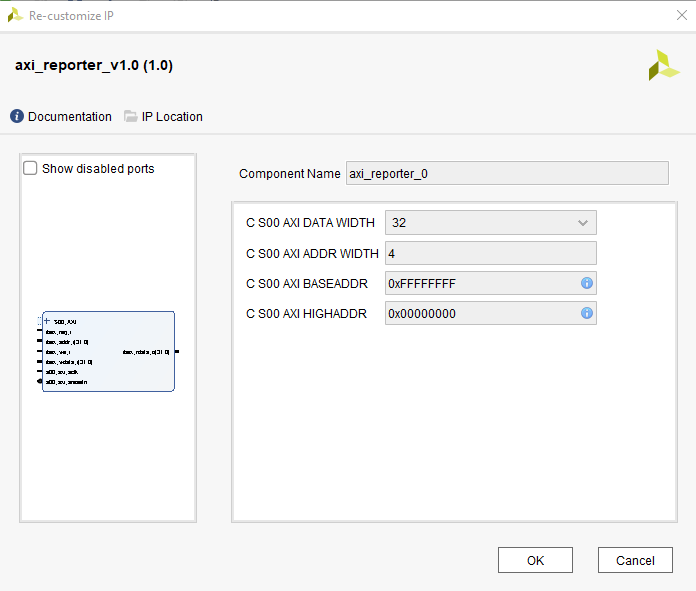
\includegraphics[width=0.8\textwidth]{axi_report.png}
    \caption{Interfaz de personalización del bloque \texttt{axi\_reporter\_0} en el entorno Vivado.}
    \label{fig:axi_reporter_config}
\end{figure}

\begin{itemize}
    \item \textbf{Ancho de Datos AXI (\textit{C S00 AXI DATA WIDTH}):} Se configuró en $32$ bits, alineándose estrictamente con el bus de datos nativo del procesador RISC-V Ibex. Esta configuración permite una transferencia de datos eficiente en un único ciclo de reloj para registros de palabra completa.
    \item \textbf{Ancho de Dirección AXI (\textit{C S00 AXI ADDR WIDTH}):} Se estableció en $4$ bits. Este valor es óptimo para la cantidad de registros internos del periférico, permitiendo un acceso mapeado en memoria dentro del espacio de direccionamiento reservado para periféricos (\textit{Memory Mapped I/O}).
\end{itemize}

Desde la perspectiva del diseño, el bloque \texttt{axi\_reporter\_0} expone una interfaz de señales que incluye las líneas de control (\textit{req}, \textit{we}, \textit{addr}) y los buses de datos de escritura y lectura. Estas señales son interconectadas directamente con el decodificador implementado en el \textit{wrapper} (\texttt{ibex\_bram\_subsystem.sv}), permitiendo que el núcleo RISC-V acceda al periférico cuando la dirección de acceso se encuentra dentro del rango lógico definido por la señal \texttt{sel\_ts}.

Esta modularidad permite que, ante la necesidad de futuras actualizaciones o escalabilidad del sistema de reporte, se puedan modificar los registros internos del \textit{Reporter} sin alterar la jerarquía superior del procesador o la estructura de la memoria BRAM.
\section{Implementación del Diagrama de Bloques (\textit{Block Design})}
Una vez configurados los módulos HDL personalizados y empaquetados los núcleos IP, el paso final del flujo de diseño consistió en la integración del sistema dentro del entorno gráfico de \textit{Block Design} de Vivado. Esta etapa permite la interconexión visual de los componentes, la gestión de las señales de reloj y reset, y el mapeo de interfaces con la arquitectura del sistema en chip (SoC).

El diseño global se estructuró incorporando los siguientes componentes clave y directrices de interconexión:

\begin{enumerate}
    \item \textbf{Distribución de Relojes (\textit{Clock Distribution}):} Se conectó la salida principal de reloj \texttt{FCLK\_CLK0} del bloque \textit{ZYNQ7 Processing System} (configurada a una frecuencia estable de 50 MHz) hacia los pines de reloj de todos los bloques IP subsiguientes y del subsistema del Ibex, garantizando un dominio de reloj síncrono en toda la lógica programable (PL).
    \item \textbf{Control de Periféricos mediante AXI GPIO:} Se añadieron dos bloques \textit{AXI GPIO} independientes para tender un puente de control y comunicación desde el Zynq Processing System hacia el resto de los componentes en la PL:
    \begin{itemize}
        \item \textbf{GPIO 0 (Gatillo de Reset):} Destinado a gobernar de manera externa y condicional la línea de reinicio activo en bajo (\texttt{rst\_ni}) del procesador Ibex.
        \item \textbf{GPIO 1 (Depuración Visual):} Utilizado como canal auxiliar de salida para la visualización de estados lógicos mediante indicadores físicos (LEDs) de la placa Zybo.
    \end{itemize}
    \item \textbf{Controlador de Memoria (\textit{AXI BRAM Controller}):} Se incorporó este IP para mediar entre el bus AXI del sistema de procesamiento ARM y el puerto de acceso dual (Puerto A) de la memoria interna BRAM. Su función principal es traducir las transacciones de lectura y escritura emitidas por Linux en accesos estructurados sobre la memoria de instrucciones y datos del procesador RISC-V durante las fases de inyección y arranque.
    \item \textbf{Gestión de Sincronismo con \textit{Processor System Reset}:} Se integró este bloque para monitorear las señales de bloqueo (\textit{locked}) del sistema y las fuentes de alimentación, generando los pulsos de reseteo sincronizados adecuados para los distintos dominios lógicos y buses del diseño.
    \item \textbf{Ruteo de Tráfico con \textit{AXI Interconnect}:} Se empleó este conmutador centralizado para arbitrar, decodificar y enrutar las peticiones provenientes del procesador ARM hacia los diferentes periféricos mapeados en memoria (Controlador BRAM, GPIOs y el Módulo Reporter).
    \item \textbf{Instanciación del Bloque \textit{Wrapper} y el \textit{AXI Reporter}:} Se importó el módulo principal \texttt{ibex\_bram\_wrapper\_bd} junto al IP \texttt{axi\_reporter\_0}, cerrando la topología de la arquitectura propuesta.
\end{enumerate}

\section{Mapeo e Interconexión de Interfaces del Sistema}
Para garantizar la interoperabilidad entre el sistema de procesamiento ARM del Zynq, el núcleo RISC-V Ibex y el periférico de monitoreo, se establecieron las rutas de interconexión a nivel de pines y buses dentro del entorno de diseño. Las siguientes tablas detallan las asignaciones y dependencias de señal configuradas en la topología de hardware.

\subsection{Conexiones del Sistema y Distribución de Relojes}
El suministro de la señal de reloj principal (\texttt{FCLK\_CLK0}) y la gestión centralizada de los pulsos de reinicio (\textit{reset}) se distribuyen de manera síncrona a todos los bloques IP conectados en la lógica programable (PL), tal como se detalla en las Tablas \ref{tab:autogenate conexion} y \ref{tab:clock_reset}.

%\begin{table}[!ht]
%    \centering
%    \caption{Conexiones autogeneradas del sistema AXI.}
%    \label{tab:autogenate conexion}
%    \begin{tabular}{|l|l|l|l|}
%    \hline
%        Bloque de origen & Pin de origen & Bloque de destino & Pin de destino \\ \hline
%        processing\_system7\_0 & M\_AXI\_GP0\_ACLK & processing\_system7\_0 & FCLK\_CLK0 \\ \hline
%        processing\_system7\_0 & M\_AXI\_GP0\_ACLK & rst\_ps7\_0\_50M & slowest\_sync\_clk \\ \hline
%        processing\_system7\_0 & M\_AXI\_GP0\_ACLK & axi\_reporter\_0 & s00\_axi\_aclk \\ \hline
%        processing\_system7\_0 & M\_AXI\_GP0\_ACLK & ps7\_0\_axi\_periph & ACLK \\ \hline
%        processing\_system7\_0 & M\_AXI\_GP0\_ACLK & ps7\_0\_axi\_periph & S00\_ACLK \\ \hline
%        processing\_system7\_0 & M\_AXI\_GP0\_ACLK & ps7\_0\_axi\_periph & M00\_ACLK \\ \hline
%        processing\_system7\_0 & M\_AXI\_GP0\_ACLK & ps7\_0\_axi\_periph & M01\_ACLK \\ \hline
%        processing\_system7\_0 & M\_AXI\_GP0\_ACLK & ps7\_0\_axi\_periph & M02\_ACLK \\ \hline
%        processing\_system7\_0 & M\_AXI\_GP0\_ACLK & axi\_gpio\_0 & s\_axi\_aclk \\ \hline
%        processing\_system7\_0 & M\_AXI\_GP0\_ACLK & axi\_gpio\_1 & s\_axi\_aclk \\ \hline
%        processing\_system7\_0 & M\_AXI\_GP0\_ACLK & axi\_bram\_ctrl\_0 & s\_axi\_aclk \\ \hline
%        processing\_system7\_0 & FCLK\_RESET0\_N & rst\_ps7\_0\_50M & ext\_reset\_in \\ \hline
%        processing\_system7\_0 & M\_AXI\_GP0 & ps7\_0\_axi\_periph & S00\_AXI \\ \hline
%        processing\_system7\_0 & FIXED\_IO & external port & FIXED\_IO \\ \hline
%        processing\_system7\_0 & DDR & external port & DDR \\ \hline
%        processing\_system7\_0 & FCLK\_CLK0 & ibex\_bram\_wrapper\_bd\_0 & bram\_clk\_a \\ \hline
%        rst\_ps7\_0\_50M & peripheral\_aresetn & ps7\_0\_axi\_periph & ARESETN \\ \hline
%        rst\_ps7\_0\_50M & peripheral\_aresetn & ps7\_0\_axi\_periph & S00\_ARESETN \\ \hline
%        rst\_ps7\_0\_50M & peripheral\_aresetn & ps7\_0\_axi\_periph & M00\_ARESETN \\ \hline
%        rst\_ps7\_0\_50M & peripheral\_aresetn & ps7\_0\_axi\_periph & M01\_ARESETN \\ \hline
%        rst\_ps7\_0\_50M & peripheral\_aresetn & ps7\_0\_axi\_periph & M02\_ARESETN \\ \hline
%        rst\_ps7\_0\_50M & peripheral\_aresetn & ps7\_0\_axi\_periph & M03\_ARESETN \\ \hline
%        rst\_ps7\_0\_50M & peripheral\_aresetn & axi\_gpio\_0 & s\_axi\_aresetn \\ \hline
%        rst\_ps7\_0\_50M & peripheral\_aresetn & axi\_gpio\_1 & s\_axi\_aresetn \\ \hline
 %       rst\_ps7\_0\_50M & peripheral\_aresetn & axi\_bram\_ctrl\_0 & s\_axi\_aresetn \\ \hline
%        ps7\_0\_axi\_periph & M00\_AXI & axi\_gpio\_0 & S\_AXI \\ \hline
%        ps7\_0\_axi\_periph & M02\_AXI & axi\_gpio\_1 & S\_AXI \\ \hline
%        ps7\_0\_axi\_periph & M03\_AXI & axi\_bram\_ctrl\_0 & S\_AXI \\ \hline
%    \end{tabular}
%\end{table}

%\begin{table}[!ht]
%    \centering
%    \caption{Conexiones específicas de reloj y reset del sistema.}
%    \label{tab:clock_reset}
%    \begin{tabular}{|l|l|l|l|}
%    \hline
%        Bloque de origen & Pin de origen & Bloque de destino & Pin de destino \\ \hline
%        processing\_system7\_0 & FCLK\_CLK0 & ibex\_bram\_wrapper\_bd\_0 & clk\_i \\ \hline
%        processing\_system7\_0 & FCLK\_CLK0 & ibex\_bram\_wrapper\_bd\_0 & bram\_clk\_a \\ \hline
%        processing\_system7\_0 & FCLK\_CLK0 & axi\_reporter\_0 & s00\_axi\_aclk \\ \hline
%        axi\_gpio\_0 & gpio\_io\_o & ibex\_bram\_wrapper\_bd\_0 & rst\_ni \\ \hline
%    \end{tabular}
%\end{table}

\subsection{Interfaz de Comunicación entre el Subsistema ARM y la Memoria BRAM}
Para permitir que el procesador ARM (bajo Linux) cargue las instrucciones y gestione el espacio de memoria compartido, se configuró el puente de datos reflejado en la Tabla \ref{tab:arm_bram}. Este enlace mapea el controlador AXI BRAM hacia el puerto dual del envoltorio del procesador RISC-V.

%\begin{table}[!ht]
%    \centering
%    \caption{Interconexión de la interfaz ARM con el subsistema BRAM de Ibex.}
%    \label{tab:arm_bram}
%    \begin{tabular}{|l|l|l|l|}
%    \hline
%        Bloque de origen & Pin de origen & Bloque de destino & Pin de destino \\ \hline
%        axi\_bram\_ctrl\_0 & bram\_clk\_a & ibex\_bram\_wrapper\_bd\_0 & bram\_clk\_a \\ \hline
%        axi\_bram\_ctrl\_0 & bram\_en\_a & ibex\_bram\_wrapper\_bd\_0 & bram\_en\_a \\ \hline
%        axi\_bram\_ctrl\_0 & bram\_we\_a[3:0] & ibex\_bram\_wrapper\_bd\_0 & bram\_we\_a[3:0] \\ \hline
%        axi\_bram\_ctrl\_0 & bram\_addr\_a[12:0] & ibex\_bram\_wrapper\_bd\_0 & bram\_addr\_a[12:0] \\ \hline
%        axi\_bram\_ctrl\_0 & bram\_wrdata\_a[31:0] & ibex\_bram\_wrapper\_bd\_0 & bram\_wrdata\_a[31:0] \\ \hline
%        axi\_bram\_ctrl\_0 & bram\_rdata\_a[31:0] & ibex\_bram\_wrapper\_bd\_0 & reporter\_rdata[31:0] \\ \hline
%       axi\_bram\_ctrl\_0 & bram\_rdata\_a[31:0] & ibex\_bram\_wrapper\_bd\_0 & ibex\_rdata\_o[31:0] \\ \hline
%        processing\_system7\_0 & M\_AXI\_GP0\_ACLK & ibex\_bram\_wrapper\_bd\_0 & clk\_i \\ \hline
%        axi\_gpio\_0 & gpio\_io\_i[3:0] & ibex\_bram\_wrapper\_bd\_0 & rst\_ni \\ \hline
%        axi\_reporter\_0 & ibex\_rdata\_o[31:0] & ibex\_bram\_wrapper\_bd\_0 & reporter\_rdata\_i[31:0] \\ \hline
%    \end{tabular}
%\end{table}

\subsection{Integración del Periférico de Monitoreo (\textit{AXI Reporter})}
El intercambio de marcas de tiempo y eventos de verificación en tiempo real se canaliza a través de las señales expuestas por el bloque \texttt{axi\_reporter\_0}. La Tabla \ref{tab:ibex_bram-reporter} detalla las líneas de control y buses interconectados con el envoltorio de Ibex.

%\begin{table}[!ht]
%    \centering
%    \caption{Conexiones de entrada y salida del bloque \texttt{axi\_reporter\_0}.}
%    \label{tab:ibex_bram-reporter}
%    \begin{tabular}{|l|l|l|l|}
%    \hline
%        Bloque de origen & Pin de origen & Bloque de destino & Pin de destino \\ \hline
%        ibex\_bram\_wrapper\_bd\_0 & reporter\_req\_o & axi\_reporter\_0 & ibex\_req\_i \\ \hline
%        ibex\_bram\_wrapper\_bd\_0 & reporter\_addr\_o[31:0] & axi\_reporter\_0 & ibex\_addr\_i[31:0] \\ \hline
%        ibex\_bram\_wrapper\_bd\_0 & reporter\_we\_o & axi\_reporter\_0 & ibex\_we\_i \\ \hline
%        ibex\_bram\_wrapper\_bd\_0 & reporter\_wdata\_o[31:0] & axi\_reporter\_0 & ibex\_wdata\_i[31:0] \\ \hline
%        ps7\_0\_axi\_periph & M01\_AXI & axi\_reporter\_0 & S00\_AXI \\ \hline
%        processing\_system7\_0 & FCLK\_CLK0 & axi\_reporter\_0 & s00\_axi\_aclk \\ \hline
%        rst\_ps7\_0\_50M & peripheral\_aresetn[0:0] & axi\_reporter\_0 & s00\_axi\_aresetn \\ \hline
%    \end{tabular}
%\end{table}

\subsection{Periféricos de Entrada/Salida de Propósito General}
Finalmente, para la depuración física del sistema y la interacción con los elementos externos de la placa de desarrollo Zybo, se configuraron los canales GPIO y los puertos físicos globales listados en la Tabla \ref{tab:io_varios}.

%\begin{table}[H]
%    \centering
%    \caption{Asignación de puertos de E/S de propósito general y periféricos externos.}
%    \label{tab:io_varios}
%    \begin{tabular}{|l|l|l|l|}
%    \hline
%        Bloque de origen & Pin de origen & Bloque de destino & Pin de destino \\ \hline
%        axi\_gpio\_0 & GPIO & external port & btns\_4bits \\ \hline
%        axi\_gpio\_0 & gpio\_io\_i[3:0] & external port & gpio\_io\_i[3:0] \\ \hline
%        axi\_gpio\_1 & GPIO & external port & leds\_4bits \\ \hline
%        axi\_gpio\_1 & gpio\_io\_o[3:0] & external port & gpio\_io\_o[3:0] \\ \hline
%        axi\_bram\_ctrl\_0 & BRAM\_PORTA & axi\_bram\_ctrl\_0\_bram & BRAM\_PORTA \\ \hline
%    \end{tabular}
%\end{table}

\subsection{Validación de la Topología}
Tras completar la interconexión, se procedió a la ejecución de la validación del diseño (\textit{Validate Design}). Este proceso verifica que no existan puertos desconectados, conflictos de asignación de direcciones o problemas de ancho de banda en los buses. 

Una vez validada la topología, se generó el producto de salida (\textit{Generate Output Products}) y el archivo de nivel superior (\textit{Create HDL Wrapper}), el cual permite que el entorno de Vivado sintetice la jerarquía completa del sistema para su posterior implementación en la FPGA, finalizando así la construcción del entorno hardware propuesto para la presente tesis. Ver \ref{fig:vivado_block_design}.

%\begin{figure}[!ht]
%     \centering
%     \includegraphics[width=1.09\textwidth]{figs/design_3_recortado.pdf}
%     \caption{Vista general del \textit{Block Design} integrado en Vivado.}
%     \label{fig:block_design}
%\end{figure}

\section{Proceso de Síntesis, Implementación y Generación del Bitstream}
Una vez concluida la interconexión lógica de los bloques y aplicado el archivo de restricciones físicas (\texttt{.xdc}), el entorno de desarrollo AMD Vivado ejecuta las fases de traducción del diseño de alto nivel hacia la estructura de silicio específica de la FPGA Zybo Z7 (modelo \texttt{xc7z010clg400-1}). Este proceso secuencial comprende las siguientes etapas críticas:

\begin{enumerate}
    \item \textbf{Síntesis del Diseño (\textit{Synthesis}):} En esta fase, Vivado analiza el código HDL del subsistema Ibex, los bloques wrapper y los IPs interconectados en el Diagrama de Bloques, transformando la descripción de hardware en una lista de conexiones netlist compuesta por primitivas lógicas de Xilinx (compuertas, multiplexores y celdas de memoria BRAM). Durante este proceso se optimiza la lógica combinacional y secuencial sin alterar la funcionalidad del sistema.
    \item \textbf{Implementación del Sistema (\textit{Implementation}):} Esta etapa se divide a su vez en tres subprocesos fundamentales:
    \begin{itemize}
        \item \textit{Optimizaciones y Mapeo (\textit{Opt Design \& Map}):} Ajusta el netlist a los recursos físicos disponibles en la FPGA, agrupando las celdas lógicas dentro de los bloques lógicos configurables (CLBs).
        \item \textit{Ruteo y Colocación (\textit{Place and Route - P\&R}):} Asigna ubicaciones físicas exactas a cada componente dentro de la matriz de silicio y establece las conexiones de interconexión metálica (\textit{routing}), respetando estrictamente las restricciones temporales de los relojes.
    \end{itemize}
    \item \textbf{Generación del Archivo de Configuración (\textit{Generate Bitstream}):} Como paso final del flujo hardware, la herramienta compila los resultados de la implementación en un archivo binario de configuración denominado \textit{bitstream} (\texttt{.bit}). Este archivo contiene la secuencia exacta de bits necesaria para configurar la matriz de celdas de la FPGA al momento del arranque.
\end{enumerate}

Paralelamente, el flujo de compilación genera el archivo de exportación de hardware en formato \textit{Xilinx Support Archive} (\texttt{.xsa}), el cual encapsula tanto la descripción física del sistema procesador ARM (PS) como los componentes de la lógica programable (PL), permitiendo la transición hacia el entorno de desarrollo de software embebido y la posterior integración del sistema operativo Linux.

\section{Adquisición e Instalación de Linux}
Para la adquisición del sistema operativo se empleó una imagen de Linux adaptada para la plataforma Zybo, obtenida a partir de los recursos de desarrollo de la comunidad \cite{miscircuitos_zybo_linux}. El almacenamiento y la ejecución del sistema se configuraron mediante una tarjeta de memoria microSD.

\subsection{Preparación de la Tarjeta SD y Verificación de Integridad}
El volcado de la imagen sobre la tarjeta SD se llevó a cabo utilizando la herramienta de software \textit{Win32 Disk Imager}. Con el fin de garantizar que la descarga del archivo comprimido se haya realizado de forma íntegra y sin corrupciones de datos, se calculó y validó el código de redundancia mediante la función hash MD5, obteniendo el siguiente valor de verificación:
\begin{equation*}
    \text{MD5: } \texttt{cbaeef7e7f551052f5451957a5dbef43}
\end{equation*}

Adicionalmente, se descargaron los archivos correspondientes al paquete \textit{kernel-zybo}, los cuales fueron descomprimidos y copiados directamente en la partición de arranque de la tarjeta SD.

\begin{figure}[h]
    \centering
    
\includegraphics[width=0.5\linewidth]{win32disk.png}
    \caption{Interfaz de selección de unidad en \textit{Win32 Disk Imager}.}
    \label{fig:win32disk}
\end{figure}

\begin{figure}[h]
    \centering
    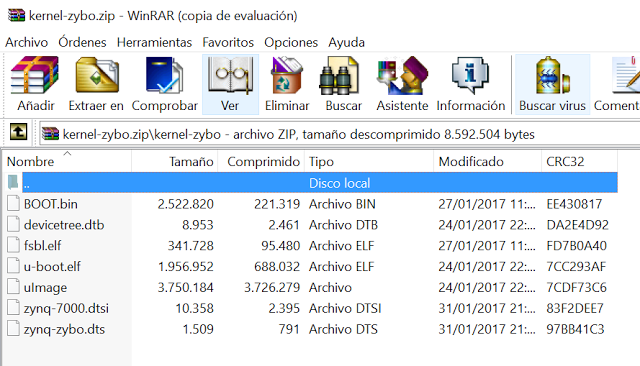
\includegraphics[width=0.5\linewidth]{figs/Archivosdekernelzybo.png}
    \caption{Estructura de archivos correspondientes al paquete \textit{kernel-zybo}.}
    \label{fig:kernel_zybo}
\end{figure}

\subsection{Configuración del \textit{Device Tree}}
A diferencia de los ordenadores de escritorio tradicionales (arquitectura x86), donde el hardware cuenta con mecanismos de auto-descubrimiento (como los buses PCI o USB), en los sistemas embebidos y microcontroladores basados en arquitectura ARM no existe un estándar nativo para que el sistema operativo detecte automáticamente los componentes periféricos integrados en la lógica programable.

Para solventar esta limitación, se configuró el archivo de descripción de hardware (\textit{Device Tree Source}, \texttt{devicetree.dts}), tomando como base el archivo \textit{zynq-zybo.dts} provisto por la placa. Su edición se realizó mediante editores de texto (\textit{Visual Studio Code} y \textit{Sublime Text}).

Por lo extenso del código, este fue incluido en el Apéndice~\ref{app:dts}.

La compilación del archivo modificado \texttt{.dts} hacia su formato binario ejecutable por el kernel de Linux (\textit{Device Tree Blob}, \texttt{.dtb}) se ejecutó desde la terminal de Linux mediante la herramienta de compilación \textit{dtc} (Device Tree Compiler):

\begin{lstlisting}[style=bashstyle]
dtc -I dts -O dtb -o devicetree.dtb devicetree.dts
\end{lstlisting}

Trabajando sobre las rutas de intercambio montadas desde el subsistema WSL, el comando se estructuró de la siguiente forma:

\begin{lstlisting}[style=bashstyle]
dtc -I dts -O dtb -o /mnt/c/location/devicetree.dtb /mnt/c/Tesis/devicetree.dts
\end{lstlisting}

Es habitual que durante la ejecución de este comando el compilador devuelva advertencias de menor relevancia (como \textit{unit\_address\_vs\_reg} o \textit{clocks\_property}). Una vez finalizado el proceso, el archivo binario resultante \texttt{devicetree.dtb} se transfirió a la partición raíz de la tarjeta SD, reemplazando la versión anterior.

\section{Generación de la Imagen de Arranque (\textit{BOOT.bin})}
Durante las fases iniciales de integración, se evaluó la posibilidad de que el propio sistema operativo Linux cargara dinámicamente el archivo de configuración bitstream (\texttt{.bit}) generado en Vivado. Sin embargo, este enfoque derivaba sistemáticamente en una condición de fallo crítico del kernel (\textit{kernel panic}). 

Como solución, se optó por estructurar un archivo de arranque consolidado (\texttt{BOOT.bin}), permitiendo que el gestor inicial cargue la arquitectura de hardware de forma simultánea al encendido de la plataforma mediante la suite \textit{Xilinx Vitis 2022.2}.

\subsection{Fase 1: Creación del Proyecto de Plataforma}
1. Se inicializó el entorno de \textit{Vitis 2022.2} seleccionando un directorio de trabajo (Workspace) limpio.\\
2. Se procedió a través de la ruta \textbf{File $\rightarrow$ New $\rightarrow$ Platform Project}.\\
3. Se asignó una denominación descriptiva al proyecto (\texttt{Zybo\_Linux\_Ibex\_Platform}).\\
4. En el apartado de especificación de hardware, se seleccionó e importó el archivo compilado \texttt{.xsa} exportado desde Vivado.\\
5. Como sistema operativo de destino se configuró el entorno \textit{standalone}, asociándolo al procesador principal \textit{ps7\_cortexa9\_0}.

\subsection{Fase 2: Creación del Proyecto de Aplicación FSBL}
1. Mediante la ruta \textbf{File $\rightarrow$ New $\rightarrow$ Application Project}, se enlazó el proyecto a la plataforma previamente generada.\\
2. Se designó el nombre \texttt{Zynq\_FSBL} seleccionando como núcleo de procesamiento el primer procesador ARM Cortex-A9.\\
3. En el selector de plantillas, se seleccionó estrictamente el entorno \textit{Zynq FSBL}.

\subsection{Fase 3: Modificaciones Críticas del Entorno (Mitigación de Errores en Drivers)}
El compilador de Xilinx Vitis presenta un error crítico de compilación (\textit{cc1.exe: fatal error: *.c: Invalid argument}) al intentar empaquetar el Board Support Package (BSP) debido a que el bloque personalizado \textit{axi\_reporter} fue declarado con controladores de software, careciendo de archivos fuente físicos `.c` en su directorio. Para neutralizar esta inconsistencia, se aplicaron dos modificaciones consecutivas:

\begin{enumerate}
    \item \textbf{Modificación del Driver en el BSP:} Se accedió a la configuración del archivo \texttt{platform.spr}, ingresando al dominio \textit{standalone\_domain} y modificando el driver correspondiente al bloque \textit{axi\_reporter\_0} a un estado nulo (\textit{none}).
    \item \textbf{Neutralización del Makefile del Driver:} El archivo \textit{Makefile} se encuentra en el directorio
\texttt{libsrc/axi\_reporter\_v1\_0/src} del BSP generado por Vitis.

    Reemplazando su contenido por rutinas vacías de ejecución controlada:

\begin{lstlisting}[style=bashstyle]
all:
	@echo "Axi Reporter IP: Skipping compilation."

libs:
	@echo "Axi Reporter IP: Skipping libs."

include:
	@echo "Axi Reporter IP: Skipping include."

clean:
	@echo "Axi Reporter IP: Skipping clean."
    \end{lstlisting}
\end{enumerate}

\subsection{Fase 4: Consolidación y Generación del \textit{BOOT.bin}}
Una vez superadas las fases de compilación de la plataforma, se invocó la herramienta de empaquetado a través de \textbf{Xilinx $\rightarrow$ Create Boot Image}, configurando el entorno para la arquitectura \textit{Zynq-7000}. 

Las particiones de arranque se integraron respetando estrictamente el siguiente orden jerárquico:
\begin{enumerate}
    \item \textbf{Bootloader (1ª Partición):} Archivo ejecutable \texttt{fsbl.elf} generado en el entorno de compilación modificado.
    \item \textbf{Bitstream (2ª Partición):} Archivo de configuración de hardware \texttt{design\_1\_wrapper.bit}, el cual contiene integrado el núcleo Ibex, la memoria BRAM con el programa precargado y el módulo de trazabilidad.
    \item \textbf{Cargador Secundario (3ª Partición):} Archivo ejecutable \textit{U-Boot} (\texttt{u-boot.elf}) destinado a la transición hacia el sistema operativo Linux.
\end{enumerate}

Finalmente, tras ejecutar la orden \textit{Create Image}, el binario resultante \texttt{BOOT.bin} fue transferido a la partición FAT32 de la tarjeta SD.

\section{Modo de Arranque por Tarjeta MicroSD}
El circuito integrado Zynq en la placa Zybo permite el arranque nativo mediante una tarjeta microSD alojada en el conector físico \textit{J4}. El procedimiento operativo para la puesta en marcha comprende las siguientes etapas:

\begin{enumerate}
    \item Formateo previo de la tarjeta microSD bajo el sistema de archivos FAT32.\\
    \item Almacenamiento del archivo unificado \texttt{BOOT.bin} en la raíz de la partición.\\
    \item Inserción de la tarjeta microSD en el conector \textit{J4} de la placa Zybo.\\
    \item Configuración de los puentes físicos (\textit{jumpers}): Colocación de un puente simple sobre el conector \textit{JP5} cortocircuitando los dos pines orientados hacia la izquierda (etiquetados como ``SD''), y selección de la fuente de alimentación mediante el conector \textit{JP7} \cite{digilent_zybo_reference_manual}.\\
    \item Alimentación y encendido del sistema, permitiendo el inicio automatizado de la imagen de arranque del sistema operativo.
\end{enumerate}